% !TEX root = ../main.tex
\section{The lead-lag graph}
\label{sec:leadlag}

In the final window (\llN{} series, $T = \llT$ weeks after seasonal differencing; Davao Occidental sits out with more than a tenth of its weeks missing), PCMCI+ keeps \textbf{\llEdges{}} lagged links between provinces at $q < \fdrQ$ (Figure~\ref{fig:leadlag} and Table~\ref{tab:edges}). Plain lagged cross-correlation with the same FDR filter keeps \textbf{\xcEdges{}}, because the 2019 national epidemic makes almost every pair of provinces move together.

The proposal's sentinel idea is therefore \textbf{weakly supported at province-week level}. The links are statistical dependencies, not evidence of transmission, and several join distant provinces. Likely reasons: weekly province totals average out local waves, four years is short for \llN{} series, and reporting artefacts dominate small provinces. Synchrony studies have found travelling dengue waves at longer time scales \parencite{vanpanhuis2015}. The MPNN-LSTM benchmark points the same way: its result does not depend on its graph.

\begin{figure}[htbp]
\centering
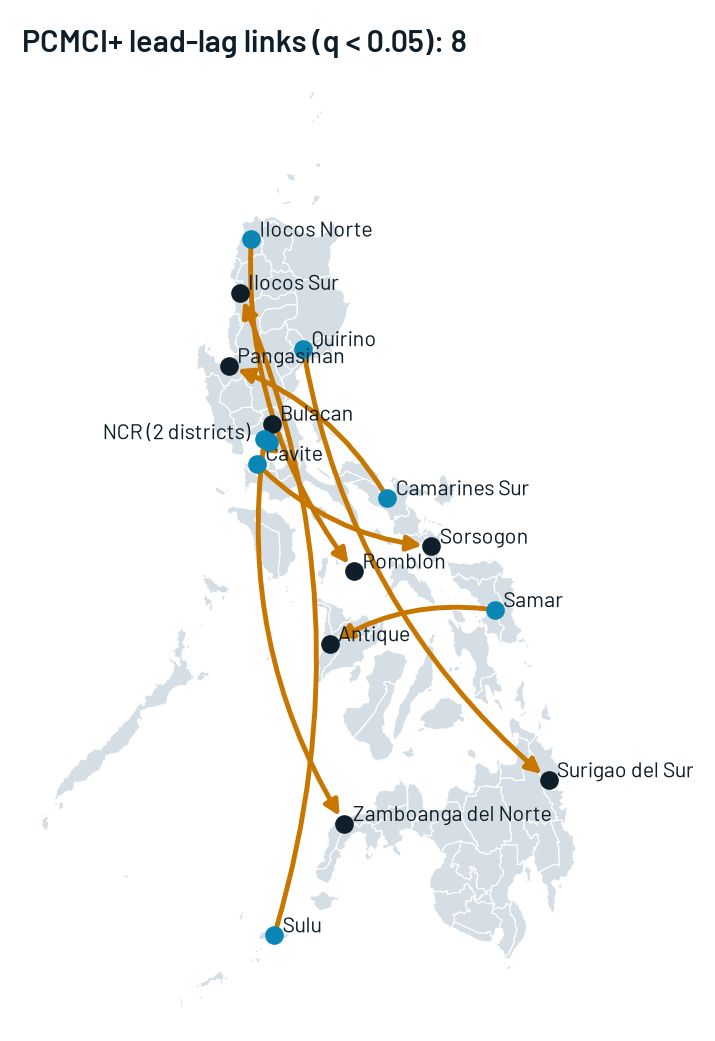
\includegraphics[width=0.48\linewidth]{f06_leadlag}
\caption{The PCMCI+ links learned on 2016--2019; teal nodes lead.}
\label{fig:leadlag}
\end{figure}

\begin{table}[htbp]
\centering
\caption{The lagged links PCMCI+ keeps, by strength: lag, partial correlation, FDR q-value and how often the link reappears over bootstrap resamples.}
\label{tab:edges}
\footnotesize
\begin{tabular}{@{}l l r r r r@{}}
\toprule
leader & follower & lag (wk) & partial corr. & $q$ & bootstrap freq. \\
\midrule
\tablerows{edges}
\bottomrule
\end{tabular}
\end{table}
